    %What the data said

    \subsection{App Test: Learning Gain and Effect of Functionality for Formative Assessment}
  There were 25 coaches active during the app test. The test clearly showed evidence between the difference between designing for Assessment and Learning. See figure \ref{fig:tabletTest} and figure \ref{fig:computerTest} to understand the setting.

  Before the quiz started, the coaches were asked to raise their hand if they felt proficient with using a smart phone. 8 out of 23 said yes. After using the app, 16 thought they were proficient (25\% increase), while 5 said low proficiency, and 2 said no (we don't yet feel proficient, still fear).

  The test was done in pairs, because of lack of devices. Manual data collection of quiz results was not viable with coaches more than 10 people (as Josefina said in Zambia), it got too hectic, which is why not all quiz results were recorded, only when coaches raised their hands, which they often did only when they got 100\%, and some never raised their hand. The results gathered can be seen in figure \ref{fig:iteration3data}. Finally, the live quiz after the app test, to evaluate the low-fidelity prototype of including open-ended questions, proved to be great for learning, and proved possible to be a great addition to the high-fidelity material.

  A couple of notes can be made from the quantitative data. Comparing quiz results between different characteristics however, some conclusions can be made. 6 groups consisted of two CBTs, and 5 groups were mixed (1 CBT and 1 Youth Mentor in the group). Among the CBT groups, the average score on a quiz was 77\%, while the presence of a Youth Mentor increased the average to 98\%. The groups were free to choose whichever quiz they wanted to. Only one group chose to redo the same quiz (scoring 100\% both times), while all others varied between different quizzes. Out of 18 quiz instances, 85\% was the mean (versus a 89\% average over 105 instances in Zambia), with 1 instance of 0\% (0/15!), 35\%, 53\%, 71\%, 2 instances of 83\%, and 12 instances of 100\%. The lower result than in Zambia could be that in Zambia the topics were still fresh, and that in Uganda, much of the information from the earlier topics of the training has not been repeated in a long time.

  Regarding pre-knowledge and learning, only 2/18 were 100\% correct on their first try, which shows the importance of feedback to improve. Only 2/12 gave up before getting 100\% on a quiz. For those that continued, 3 groups got 100\% correct on their 2nd try, 3 on the 3rd try, 2 on the 4th try, and 1 on the 6th try (meaning more coaches pass the quiz on earlier than later tries). It is difficult to see if there are major differences in quiz difficulty, as the sample of doing the individual quizzes are so low. On both the topic quiz and coach guide quiz for week 9, it can be seen that all groups eventually scored 100\%, as well as 3/4 for week 8. This may be explained by that most of the coaches were carrying out week 8, 9 or 10 at the time of the app test.

  \begin{figure}[h]
    \centering
    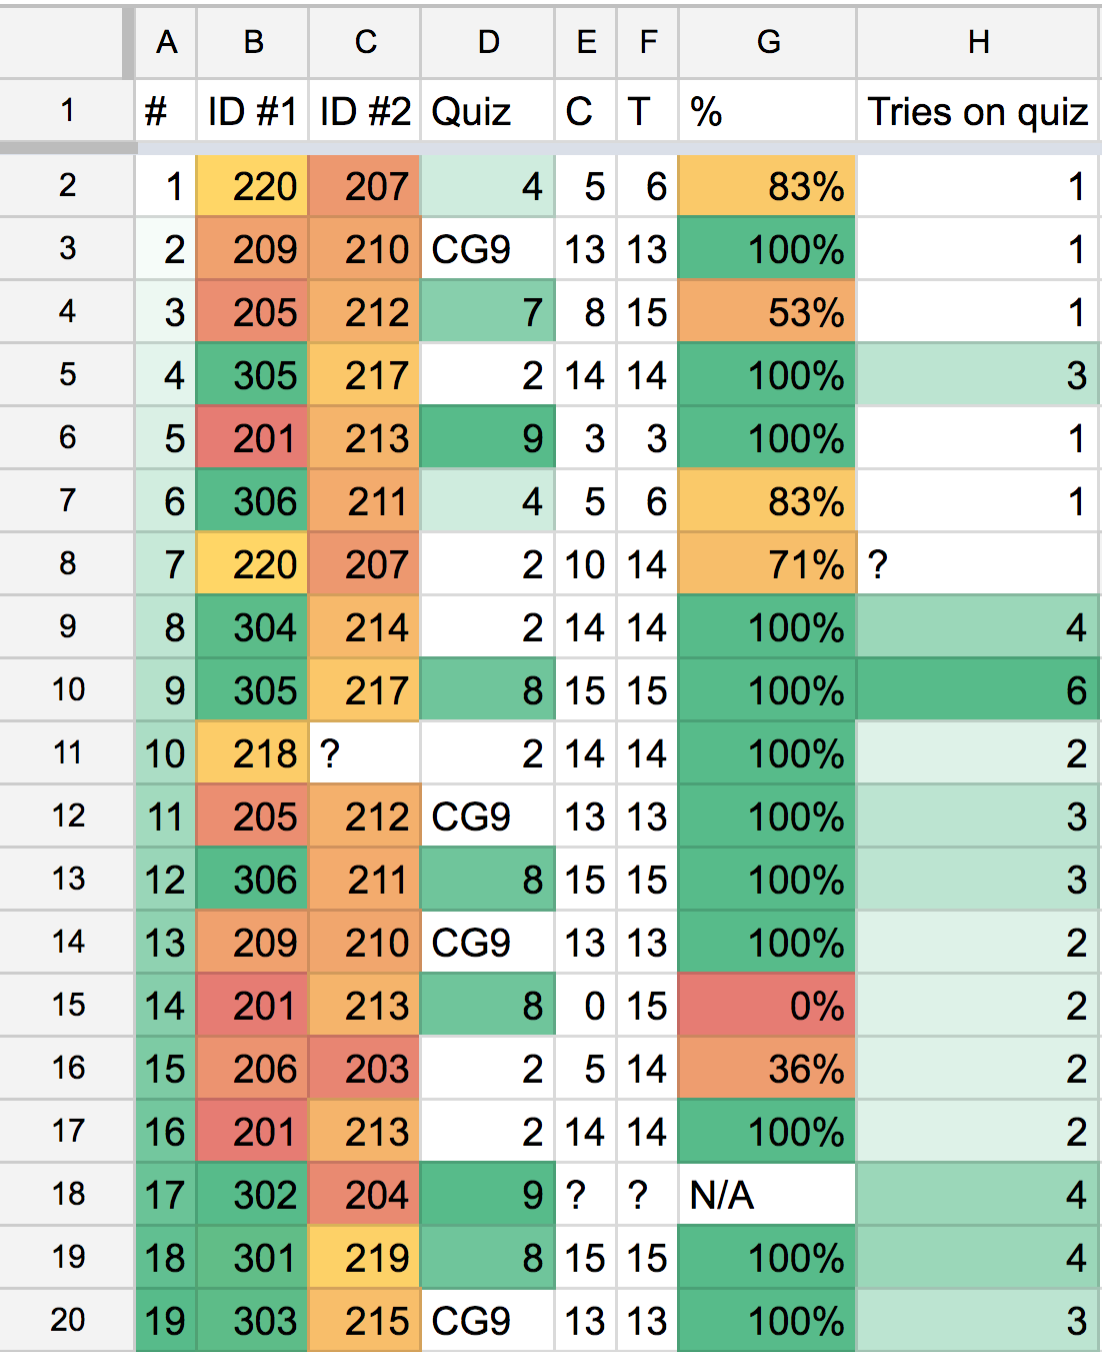
\includegraphics[width=0.8\textwidth]{analysis/iteration3data.png}
    \caption{The data gathered from iteration 3. A is order of quiz submission, B and C is Coach ID for coach 1 and 2 in the group, C is quiz chosen (CS9 meaning "Coach guide week 9"), D is correct answers, E is number of questions, G is percentage correct answers, and F is recorded quiz try on the particular topic at the time of submission.}
    \label{fig:iteration3data}
  \end{figure}

  Because the quizzes were carried out in pairs, the results are non-traceable to individuals, and thus also to pre-knowledge about the coaches or the results for iteration 4. This means it is hard to track how their results compare over time. However, the insights from this data can guide research for future workshops, interviews and app observations. %However, if is not significantly limiting for analyzing the difficulty level of the questions.

  \begin{figure}[h]
    \centering
    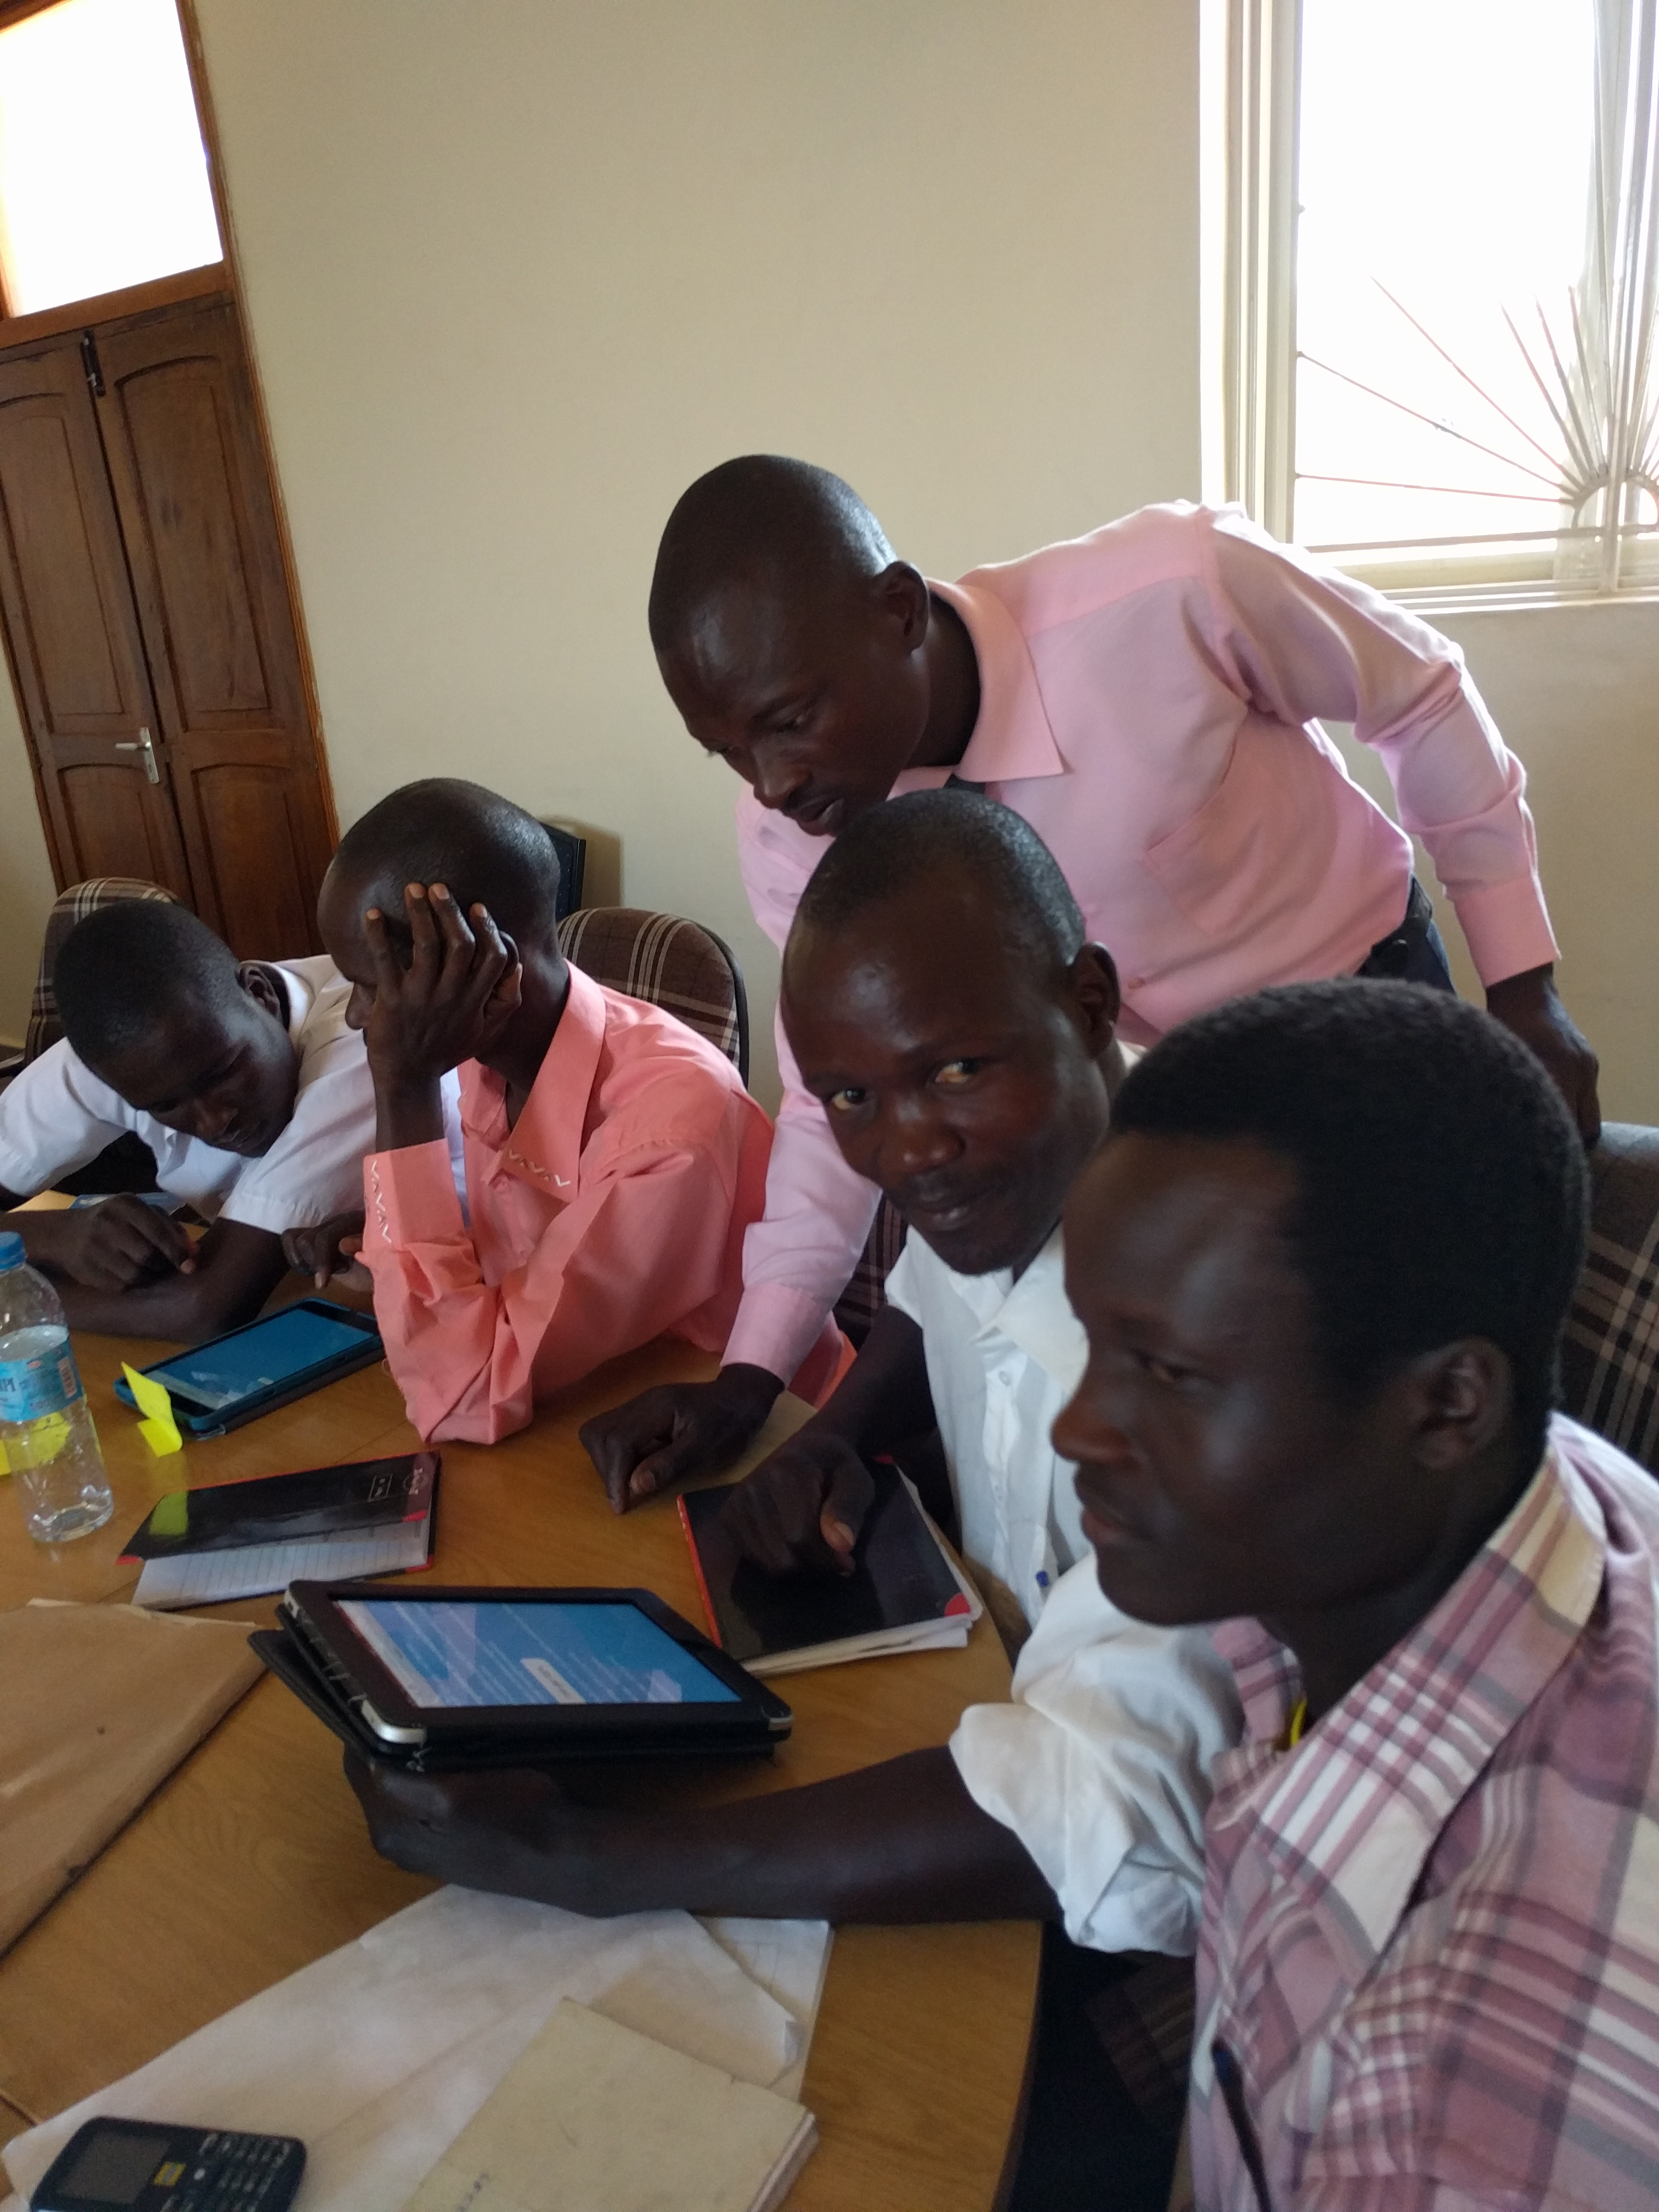
\includegraphics[width=0.4\textwidth]{iteration3/appTestTablet.jpg}
    \caption{Two coaches using a tablet for the formative app test. The coaches worked in pairs. After the app test, interviews was held, before co-creation workshops started.}
    \label{fig:tabletTest}
  \end{figure}

  \begin{figure}[h]
    \centering
    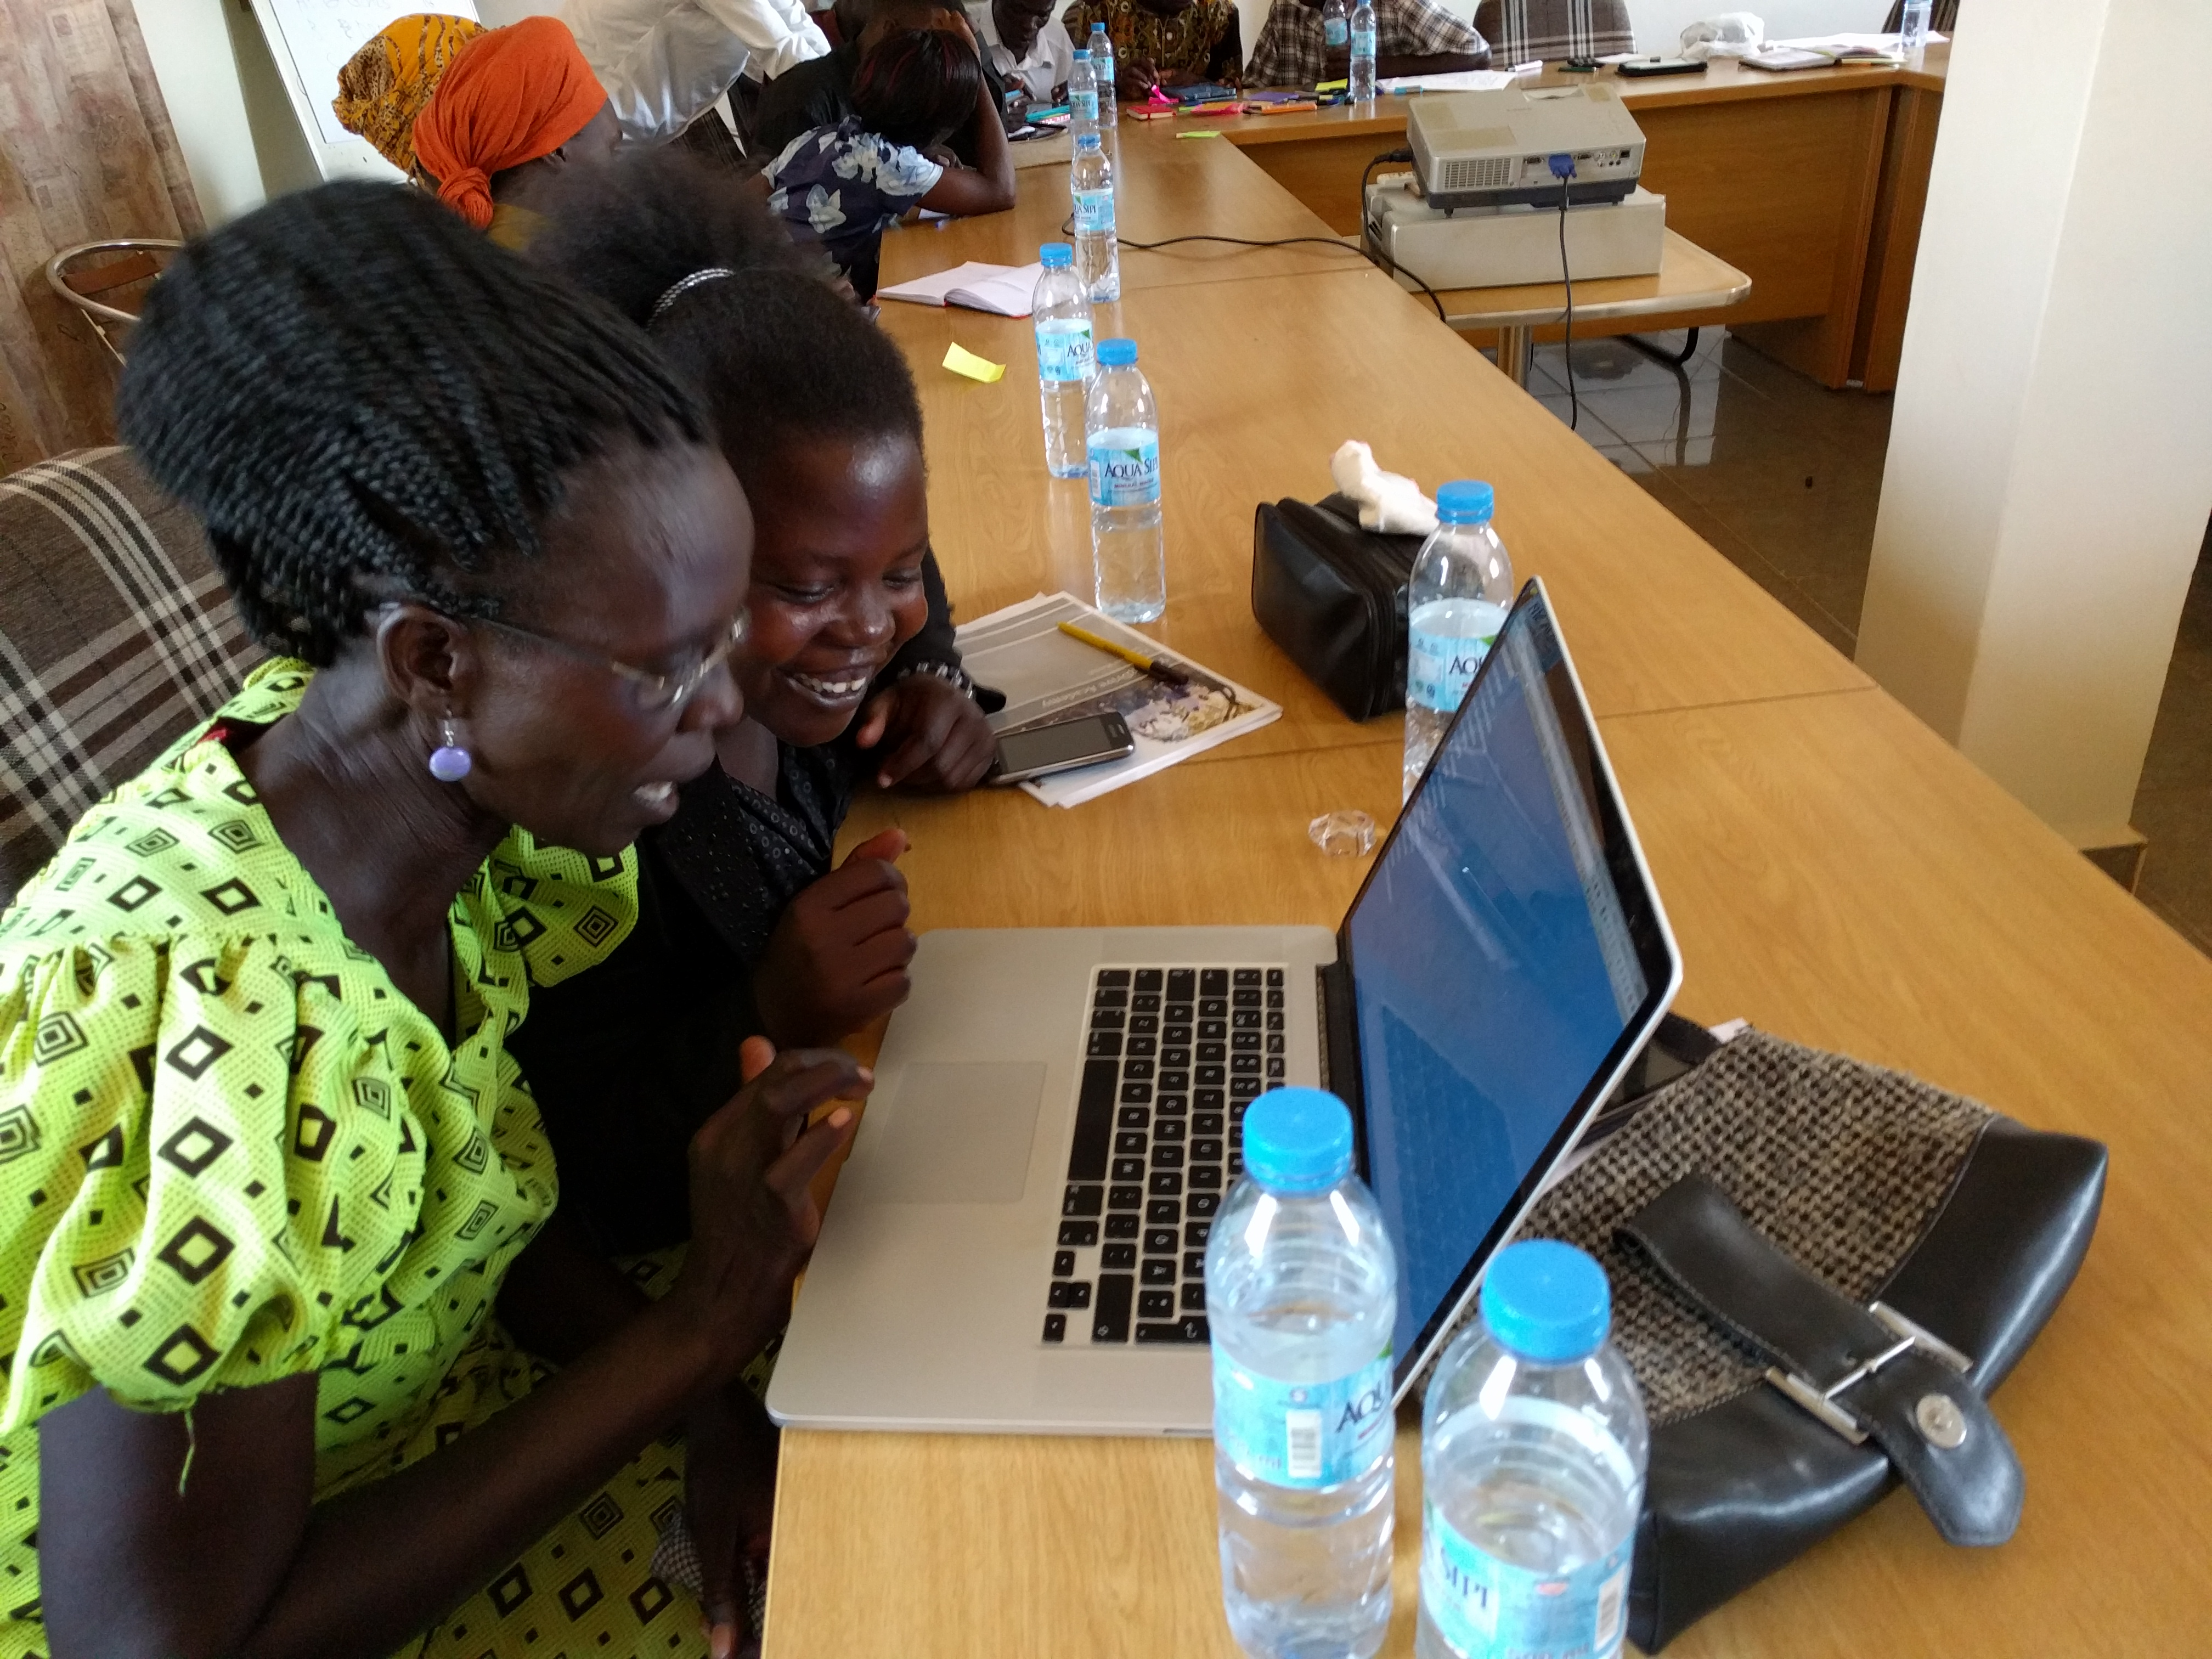
\includegraphics[width=0.8\textwidth]{iteration3/appTestComputer.jpg}
    \caption{A variation of smartphones and tablets were used. In one case, the battery died on one of the device so it needed to be replaced with a computer. It was the first time the coaches used a computer, and they learned quickly and eagerly.}
    \label{fig:computerTest}
  \end{figure}

  \subsubsection{Observations during test-session}

  Regarding usability, the most negative thing from the app test, was that the app was not user-friendly for first-time smartphone users. There were a lot of bugs, the most damaging for the app test being resizing of the font size for each new question, see figure \ref{fig:iteration-map} E-3. This forced some coaches to try to zoom on the devices, even if they did not know how. This could in turn cause a refresh of the web page, and sometimes there was no Internet available. Thus, this can explain why some quiz tries were started but never finished.

  This was the first time true frustration was shown. Out of 23 respondents, 7 rated the app easy, 11 medium, and 6 hard. This was not viable, in terms of reaching YoungDrive's goal with the app: "It should be easy to understand, pedagogical and enjoyable to use, and the coaches should think it is fun and meaningful to learn via the app", see section \ref{sec:definitionofsuccess}).

  Another reason for the low usability, is that cognitive load seemed to be too high. The feedback was not scaffolded enough, so coaches did not have enough energy to assess all of their results carefully before taking the test again via "Improve". One user did not want to press "Improve" until having read the manual. The motivation was: "Not because that is what the info says, but because I can learn more from the manual, about more than what the questions says." This is in fact the preferred behaviour from Josefina, and the app should continue to further encourage only using the app training or certification mode after having prepared via the manual. This way, the app is still assessment, but it is "learning by thinking", with feedback. In iteration 4, comparing those that are allowed to use the manuals with those that are not allowed to, would be interesting.

  Regarding learning, four new ideas were tested during the app test, assessing the new pedagogical model of the app. Item 1-3 were tested in the app (the high-fidelity trigger material), see figure \ref{fig:iteration-map}, and item 4 was tested via low-fidelity trigger material, asking a coach (and then the coach audience) if he or they could give the answers from memory without being shown alternatives.

  \begin{enumerate}
  \item "Try again"-button. When clicked, your wrong answers are repeated.
  \item If 100\% on the 1st try, gold. On 2nd try: silver. On 3rd try: bronze.
  \item Ask meta-cognitive questions, "Are you sure?", at the end of each question.
  \item Speak your answer to the question before you are shown alternatives.
  \end{enumerate}

  Item 1, 2 and 3 were determined good after the interviews. Item 4 showed relevance, but implementation in the app would give many challenges (mainly how to assess if the coach could give the right answer without giving different alternatives. Voice recognition or free-form answers are hard to analyze, to implement, and to use by a first-time smartphone user).

  \clearpage
